\documentclass[12pt]{article}
\usepackage{kerkis}
\usepackage{sfmath}
\usepackage{geometry}


\geometry{landscape, 
  left=0in,
  top=0in,
  textheight=8.5in,
  textwidth=11in,
  marginparsep=0in,
  marginparwidth=0in}


\renewcommand{\familydefault}{\sfdefault}
%\usepackage[scaled]{uarial}
%\renewcommand{\rmdefault}{phv} % Arial
%\renewcommand{\sfdefault}{phv} % Arial
%\renewcommand*\familydefault{\sfdefault} %% Only if the base font of the document is to be sans serif
%\usepackage[T1]{fontenc}
\RequirePackage{tikz,pgfplots}


\pagecolor{white!25!black!90!blue!95!green} % Color of the page
\color{white} % Color of the text
\newcommand{\surfaceColor}{violet}
\newcommand{\surfaceColorTwo}{redyellow}
\newcommand{\sliceColor}{greenyellow}





\begin{document}
\pagenumbering{gobble}

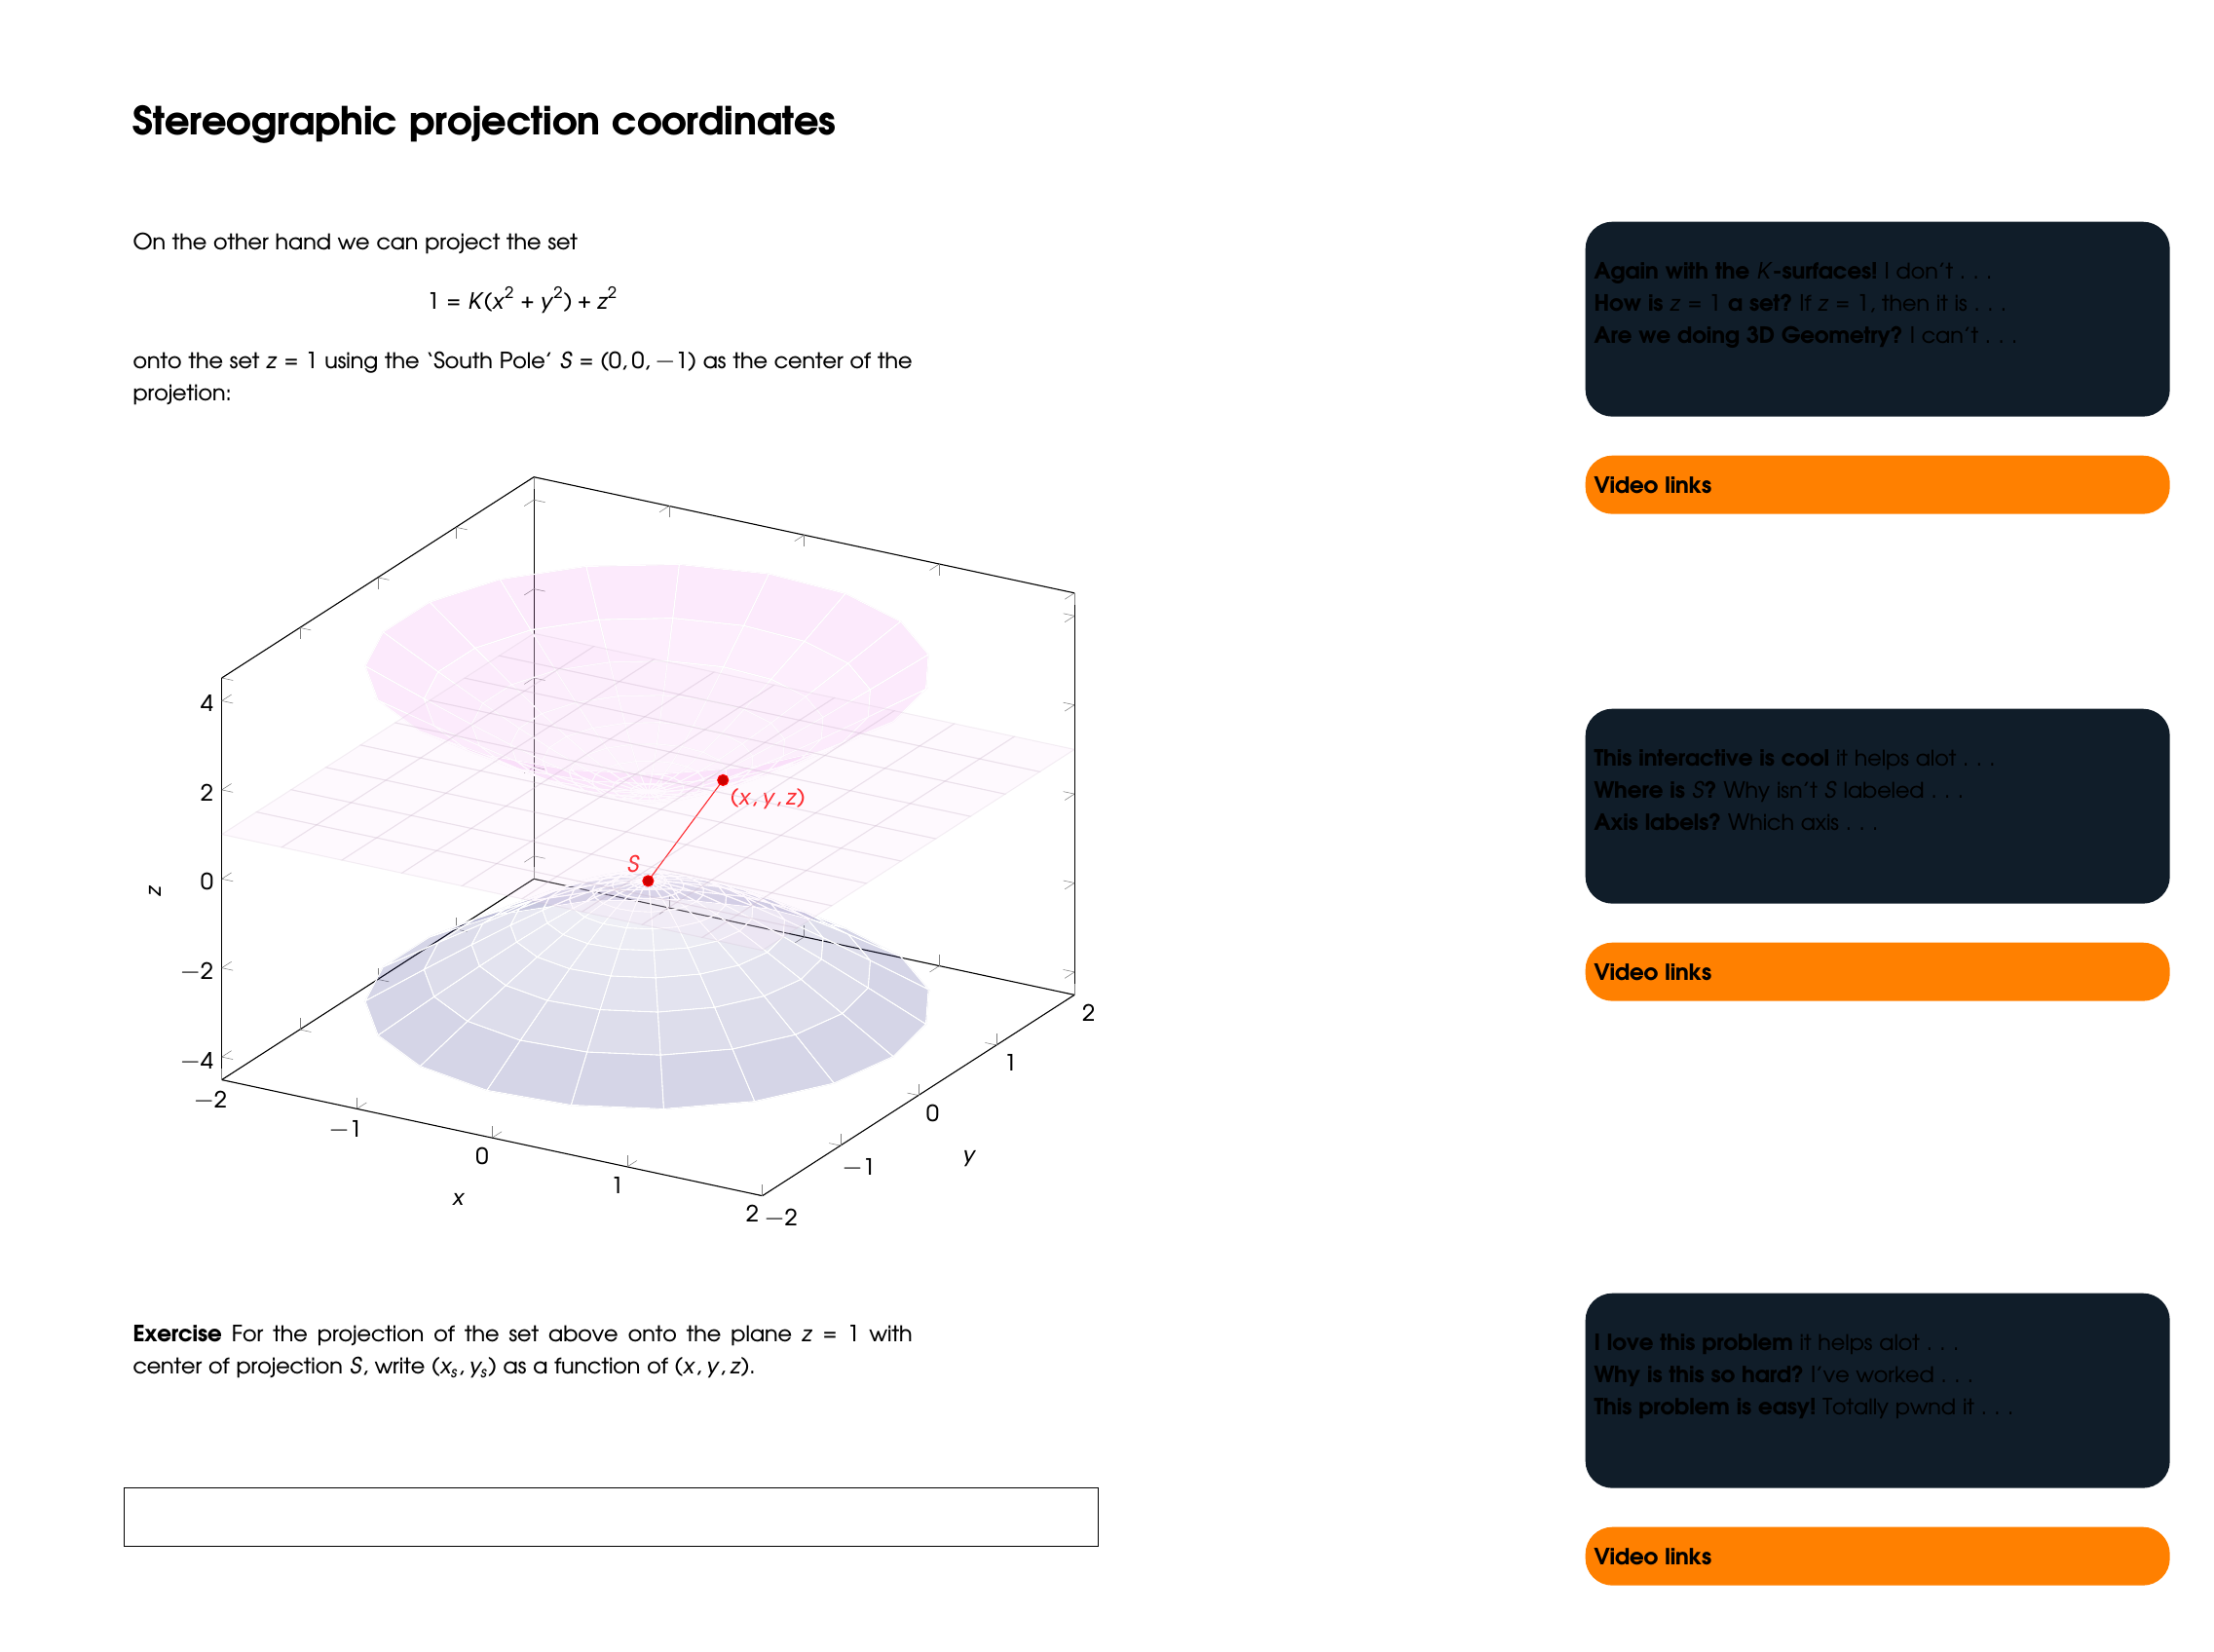
\begin{tikzpicture}

\draw[fill = none, draw=none] (0in,0in) rectangle (1in,-1in);

\draw[fill = none, draw=none] (9.5in,-7.2in) rectangle (10.5in,-8.2in);

\node[anchor=west] at (.5in, -.5in) {\scalebox{.7}{\sffamily\Huge\textbf{Stereographic projection coordinates}}};

\node[anchor=west] at (.5in, -1.5in) {
\begin{minipage}{4in}
On the other hand we can project the set
\[
1 = K(x^2+y^2) + z^2
\]
onto the set $z= 1$ using the `South Pole' $S = (0,0,-1)$ as the
center of the projetion:
\end{minipage}};


\draw[fill = black!70!white!25!black!90!blue!95!green, draw=none,rounded corners=10pt] (8in,-1in) rectangle (11in,-2in);
\node[anchor=west] at (8in, -1.5in) {
\begin{minipage}{3in}
{\bfseries Again with the $K$-surfaces!} I don't \dots\\ 
{\bfseries How is $z=1$ a set?} If $z=1$, then it is \dots\\ 
{\bfseries Are we doing 3D Geometry?} I can't  \dots\\ 
\end{minipage}};

\draw[fill = orange, draw=none,rounded corners=10pt] (8in,-2.2in) rectangle (11in,-2.5in);
\node[anchor=west,color=black] at (8in, -2.35in) {
\begin{minipage}{3in}
{\bfseries Video links} 
\end{minipage}};




\draw[fill = black!70!white!25!black!90!blue!95!green, draw=none,rounded corners=10pt] (8in,-3.5in) rectangle (11in,-4.5in);
\node[anchor=west] at (8in, -4in) {
\begin{minipage}{3in}
{\bfseries This interactive is cool} it helps alot \dots\\ 
{\bfseries Where is $S$?} Why isn't $S$ labeled \dots\\ 
{\bfseries Axis labels?} Which axis \dots\\ 
\end{minipage}};

\draw[fill = orange, draw=none,rounded corners=10pt] (8in,-4.7in) rectangle (11in,-5in);
\node[anchor=west,color=black] at (8in, -4.85in) {
\begin{minipage}{3in}
{\bfseries Video links} 
\end{minipage}};


\draw[fill = black!70!white!25!black!90!blue!95!green, draw=none,rounded corners=10pt] (8in,-6.5in) rectangle (11in,-7.5in);
\node[anchor=west] at (8in, -7in) {
\begin{minipage}{3in}
{\bfseries I love this problem} it helps alot \dots\\ 
{\bfseries Why is this so hard?} I've worked  \dots\\ 
{\bfseries This problem is easy!} Totally pwnd it \dots\\ 
\end{minipage}};

\draw[fill = orange, draw=none,rounded corners=10pt] (8in,-7.7in) rectangle (11in,-8in);
\node[anchor=west,color=black] at (8in, -7.85in) {
\begin{minipage}{3in}
{\bfseries Video links} 
\end{minipage}};






\begin{scope}[shift={(1in,-6in)}]
  \begin{axis}[
     view={30}{30},colormap/violet,
     xlabel=$x$, ylabel=$y$, zlabel=$z$,
     width=5in,
   ]

  \addplot3[surf,opacity=.2,shader=faceted,  %shade top cone
    samples=10,
    samples y =20,
    domain=0:1,y domain=0:2*pi,
    z buffer=sort]
  ({1/2 * sinh(2*x)*cos(deg(y))},{1/2 * sinh(2*x)*sin(deg(y))}, {cosh(2*x)});

 \addplot3[mesh,%opacity=.2,shader=faceted,   %mesh top cone
    draw=white,
    samples=10,
    samples y =20,
    domain=0:1,y domain=0:2*pi,
    z buffer=sort]
  ({1/2 * sinh(2*x)*cos(deg(y))},{1/2 * sinh(2*x)*sin(deg(y))}, {cosh(2*x)});






  \addplot3[surf, opacity=.2,shader=faceted,  %shade bottom cone
    draw=white,
    samples=10,
    samples y =20,
    domain=0:1,y domain=0:2*pi,
    z buffer=sort]
  ({1/2 * sinh(2*x)*cos(deg(y))},{1/2 * sinh(2*x)*sin(deg(y))}, {-cosh(2*x)});







  \addplot3[mesh,%opacity=.2,shader=faceted,  %mesh bottom cone
    draw=white,
    samples=10,
    samples y =20,
    domain=0:1,y domain=0:2*pi,
    z buffer=sort]
  ({1/2 * sinh(2*x)*cos(deg(y))},{1/2 * sinh(2*x)*sin(deg(y))}, {-cosh(2*x)});


\addplot3[red]% S to (x,y,z)
coordinates{
  (0,0,-1)
({1/2 * sinh(2*.88)*cos(deg(-.7))},{1/2 * sinh(2*.88)*sin(deg(-.7))}, {cosh(2*.88)})
};

\addplot3+[red,only marks]% S to (x,y,z)
coordinates{
  (0,0,-1)
({1/2 * sinh(2*.88)*cos(deg(-.7))},{1/2 * sinh(2*.88)*sin(deg(-.7))}, {cosh(2*.88)})
};

\node at (axis cs:0,0,-1) [red,anchor=south east] {\scalebox{1}{$S$}};
\node at (axis cs:1.07,-.908,2.99) [red,anchor=north west] {\scalebox{1}{$(x,y,z)$}};


\addplot3[surf,opacity=.2,shader=faceted,  %plane
    samples=10,
    samples y =10,
    domain=-2:2,y domain=-2:2,
    z buffer=sort]
  ({x},{y}, {1});



 \end{axis}

\end{scope}

\node[anchor=west] at (.5in, -6.8in) {
\begin{minipage}{4in}
\textbf{Exercise} For the projection of the set above onto the plane $z=1$ with center of projection $S$, write
$(x_s,y_s)$ as a function of $(x,y,z)$.  
\end{minipage}};
\draw[fill = white, draw=black] (.5in,-7.5in) rectangle (5.5in,-7.8in);



\end{tikzpicture}



\end{document}

\newpage


\pagecolor{white!20!black!80!red} % Color of the page


\subsection*{An Example of a Lune}


\begin{center}
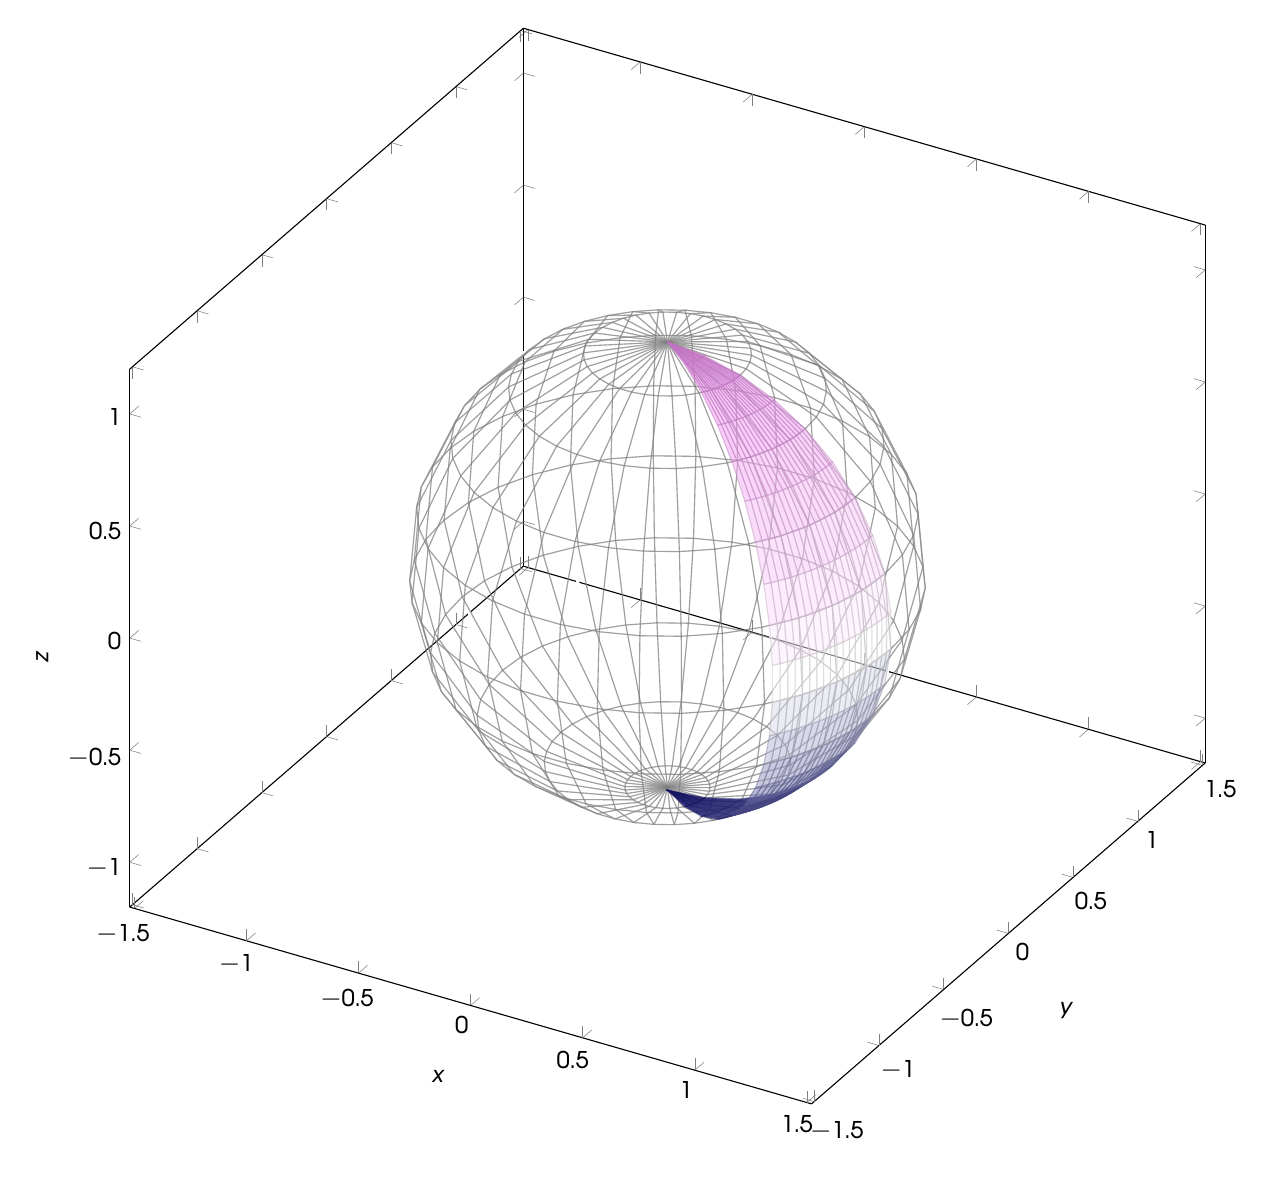
\begin{tikzpicture}
 \begin{axis}[
     view={30}{30},colormap/violet,
     xlabel=$x$, ylabel=$y$, zlabel=$z$,
     width=6in,
     height=6in,
     axis equal,
   ]
\addplot3[% lines
        mesh,
        draw=white,
        draw opacity = .7,
        thick,
        z buffer = sort,
        samples = 50,
        variable = \u,
        variable y = \v,
        domain = 0:360,
        y domain = -180:180,
    ]    
    ({cos(-36)*sin(v}, {sin(-36)*sin(v)}, {cos(v)});



\addplot3[% lines
        mesh,
        draw=white,
        draw opacity = .7,
        thick,
        z buffer = sort,
        samples = 50,
        variable = \u,
        variable y = \v,
        domain = 0:360,
        y domain = -180:180,
    ]    
    ({cos(0)*sin(v}, {sin(0)*sin(v)}, {cos(v)});

    \addplot3[% sphere itself
%        fill opacity = 0.3,
%        draw opacity = 0.0,
%        surf,
      mesh,
      draw opacity = .5,
      draw=white!50!black,
        z buffer = sort,
        samples = 20,
        variable = \u,
        variable y = \v,
        domain = 0:180,
        y domain = 0:360,
    ]    
    ({cos(u)*sin(v)}, {sin(u)*sin(v)}, {cos(v)});

\addplot3[% lune
        surf,
        opacity = 0.5,
        z buffer = sort,
        samples = 20,
        variable = \u,
        variable y = \v,
        domain = -36:0,
        y domain = 0:180,
    ]    
    ({cos(u)*sin(v)}, {sin(u)*sin(v)}, {cos(v)});





\end{axis}
\end{tikzpicture}
\end{center}

\end{document}
